\documentclass[11pt]{article}
\usepackage{charter}
\usepackage{graphicx}
\usepackage{hyperref}
\usepackage{mdframed}
\usepackage[margin=1in]{geometry}
\usepackage{amsmath,amssymb}

\hypersetup{
	colorlinks=true,
	linkcolor=blue,
	filecolor=magenta,
	urlcolor=cyan,
}

\begin{document}

%===================================================
% Title and Author Info
%===================================================
\begin{center}
{\Large\textsc{Compact Binary Inspiral and GW170817}} \\
\vspace{10pt}
{\large \textbf{Mentor:} Alex Urban} \\
{\small LIGO Laboratory, California Institute of Technology \\
Pasadena, CA 91125, USA \\
\href{mailto:aurban@ligo.caltech.edu}{\texttt{aurban@ligo.caltech.edu}}}
\end{center}

%%%%%%%%%%%%%%%%%%%%%%%%%%%%%%%%%%%%%%%%%%%%%%%%%%%

\section*{An Introduction to LIGO Astronomy}
\hspace{15pt} Suppose two neutron stars with masses $m_1 \geq m_2$ are in a stable circular orbit (see Figure \ref{fig:binary_diagram}).
As we have recently observed in the transient signal \href{https://journals.aps.org/prl/pdf/10.1103/PhysRevLett.119.161101}{GW170817}, such a
system will radiate away much of its potential energy over time in the form of gravitational waves. In this group problem set, we'll first
estimate a few observables to sketch out a back-of-the-envelope view of what merger events look like. Then, we'll look at some very real
examples of astrophysics that can be learned through gravitational wave (GW) and electromagnetic (EM) observations.

In group discussion we'll build an intuition by tinkering with some signal processing techniques, imagining how to observe this system with the
ground-based LIGO detectors. This will make use of data obtained from the \href{https://losc.ligo.org}{LIGO Open Science Center}, a service of
LIGO Laboratory, the LIGO Scientific Collaboration, and the Virgo Collaboration.

\vspace{20pt}

\begin{figure}[!h]
\begin{mdframed}
\centering
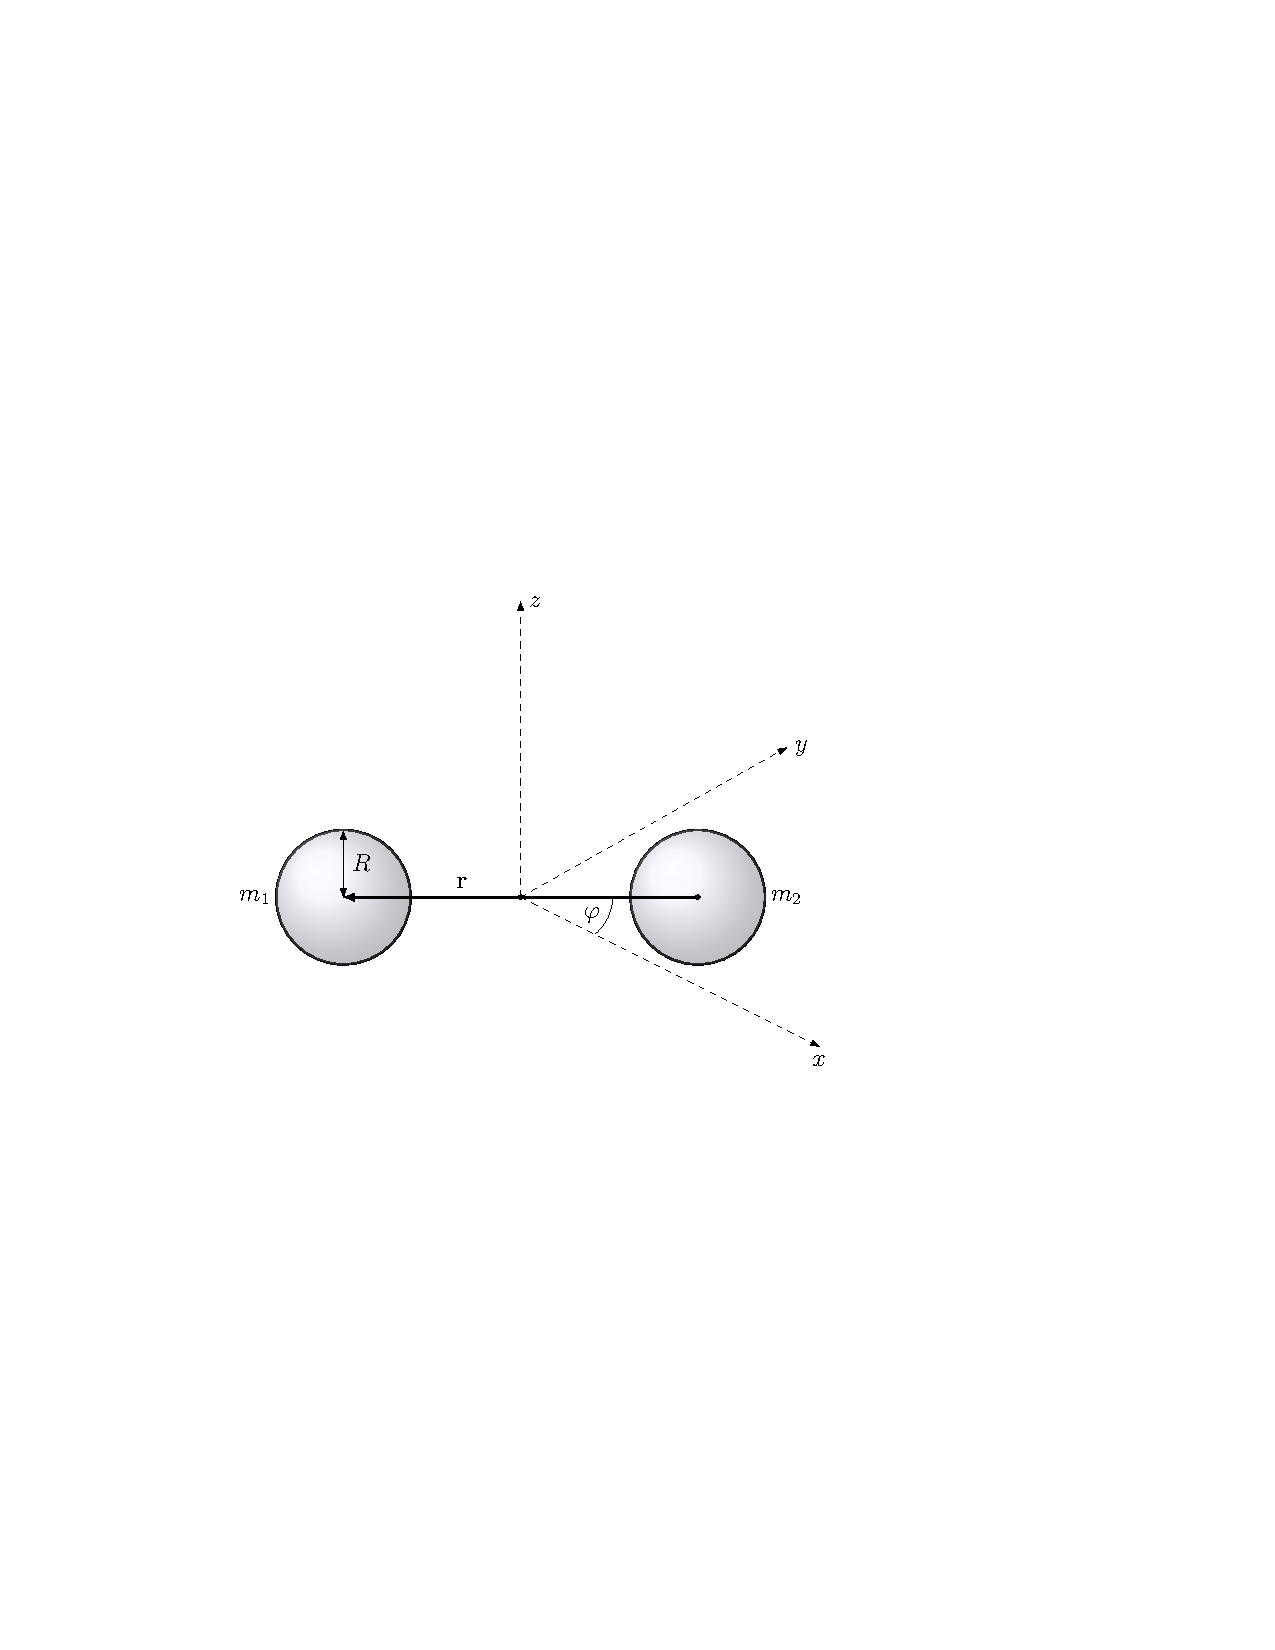
\includegraphics{intro/binary_diagram.pdf}
\caption{\label{fig:binary_diagram}Diagram of a neutron star binary in the center of mass frame, showing its orbital separation vector
($\mathbf{r}$) and the radius ($R$) and masses ($m_1 \geq m_2$) of the individual neutron stars. The orbital phase angle $\varphi$ is also
indicated.}
\end{mdframed}
\end{figure}

\vspace{1000pt}

\textbf{Note:} In what follows, $M = m_1 + m_2$ is the total mass and $\mu = m_1 m_2/(m_1 + m_2)$ is the reduced mass of the binary.

\begin{enumerate}

\item \textbf{ISCO'mplicated.} Recall that according to general relativity, it's very difficult to extract energy from this system once it reaches
the innermost stable circular orbit (ISCO), which has a separation of approximately
\begin{equation}\label{eq:rISCO}
r_{\rm ISCO} \approx \frac{6GM}{c^2}.
\end{equation} This separation is roughly the point where merger occurs.\begin{enumerate}
\item Given that $f_{\rm GW} = 2f_{\rm orbital}$, use Kepler's third law to estimate how the observed GW frequency $f_{\rm ISCO}$ at ISCO scales in
terms of $M$.

\item What are $r_{\rm ISCO}$ (in km) and $f_{\rm ISCO}$ (in Hz) if $M =$\, 2.74\,$M_{\odot}$? Where is $f_{\rm ISCO}$ relative to LIGO's sensitive
band, about 20 -- 2000 Hz?

\item What is the orbital separation when the observed signal crosses 20 Hz? How does this compare to, say, the trip from Los Angeles to San
Francisco?
\end{enumerate}

\item \textbf{The Final Countdown.} Recall that the orbital separation, $r$, shrinks over time as potential energy is lost to gravitational waves.
Consequently, the frequency sweeps up. In a previous problem set we approximated this process as
\begin{equation}\label{eq:drdt}
\frac{dr}{dt} = - \frac{64}{5} \frac{G^3}{c^5} \frac{\mu M^2}{r^3}.
\end{equation}\begin{enumerate}
\item \emph{Without} solving any differential equations, estimate how long it takes the system to evolve from an observed frequency of $f_0$ up
through merger, in terms of $\mu$ and $M$.

\item Once the signal crosses 20 Hz, how long do we have until merger if $m_1 = $\, 1.57\,$M_{\odot}$ and $m_2 =$\, 1.17\,$M_{\odot}$? How does
this compare with the observed duration ($\sim$100 s) of GW170817 in LIGO's sensitive frequency band?

\item What is the orbital velocity ($v/c$) when the observed signal is at 20 Hz? At $f_{\rm ISCO}$?
\end{enumerate}

\item \textbf{Event rates.} The LIGO detectors in Hanford, WA, and Livingston, LA, recorded data for about 49 days from Sept 2015 -- Jan 2016,
and again for about 117 days from Nov 2016 through Aug 2017. While the noise floor in each detector fluctuated greatly during this time, we can
estimate the detectors' average sensitive distance for binary neutron star mergers as 70 Mpc. In other words, as we'll discuss in group, mergers
of two neutron stars out to about this distance would produce strong enough gravitational waves to be detected by LIGO.

\begin{enumerate}
\item Given that we have observed exactly one such merger so far, what is the inferred rate of binary neutron star merger events in Gpc$^{-3}$
yr$^{-1}$?

\item What is the rate per \emph{galaxy} per year? (Assume one galaxy takes up 1 Mpc$^3$.)
\end{enumerate}

\item \textbf{We struck gold!} From EM observations\footnote{Cowperthwaite \textit{et al.},
\href{http://iopscience.iop.org/article/10.3847/2041-8213/aa8fc7}{\textit{Astrophysical Journal Letters} \textbf{848}, 2} (2017).} we have learned
that some $\sim$0.05\,$M_{\odot}$ of ejecta were released during an explosive kilonova after the merger event. It has been suspected for some time
that explosions like this produce most of the elements heavier than iron (such as gold, silver, and platinum) in the universe. Assuming this one
event is representative, how much material do neutron star mergers produce per galaxy each year? How does this compare with the estimated rate of
heavy element synthesis, 10$^{-\text{7}}$\,$M_{\odot}$ yr$^{-1}$, in the Milky Way? What uncertainties are there in these estimates?

\end{enumerate}

\end{document}
